
\documentclass[12pt]{article}
\usepackage{amsmath, amssymb, graphicx, geometry}
\geometry{margin=1in}

\title{Structured Rattling and Harmonic Resonance as Predictors of Prime Distribution in Modular Fields}
\author{Casey Allard \and ChatGPT (co-author)}
\date{\today}

\begin{document}

\maketitle

\begin{abstract}
We propose a novel framework for understanding the distribution of prime numbers based on biased stochastic motion through modular matrices. Inspired by emergent behaviors in entropy-driven systems and harmonic field resonance, we model primes as attractors within recursive modular spaces. Using rattling agents---stochastic walkers influenced by local prime entropy and $\phi$-aligned harmonic nodes---we predict zones of probable prime emergence. Our results provide a spatially structured alternative to classical sieve and probabilistic prime models, offering both visual and computational insights into prime localization.
\end{abstract}

\section{Introduction}
Prime numbers remain one of the most foundational yet elusive constructs in number theory. While classical models such as the Sieve of Eratosthenes, Cram\'er\'s probabilistic model \cite{cramer1936}, and the Riemann Hypothesis offer powerful perspectives, none provide a fully spatial or modular interpretation.

This paper introduces a modular matrix environment in which primes are treated as emergent features within a field governed by entropy and resonance. We show that a system of biased walkers---termed \textit{rattling agents}---naturally localizes in regions predictive of prime behavior, particularly in conjunction with $\phi$-resonant harmonic alignments.

\section{Modular Matrix Field Construction}
We define a modular matrix $M(i,j) = (i \cdot d + j + 1) \mod n$, where $d$ is the dimension and $n$ the modulus base. A binary prime mask identifies primes within this space. The entropy field $E(i,j)$ is defined as the inverse local prime density using a uniform kernel \cite{reich1996entropy}.

\section{Rattling Agent Dynamics}
A rattling agent is a stochastic walker that transitions toward higher entropy values, with a preference given by a tunable bias parameter $\alpha$. The walker samples its neighborhood and probabilistically selects a direction proportional to $E^\alpha$ \cite{wolf1997prime}.

\section{Entropy Field and Curvature}
We define the entropy curvature using the Laplacian $\nabla^2 E$, which identifies attractor basins where local entropy is minimized. These regions serve as natural convergence zones for rattling agents.

\section{Harmonic Alignment}
The golden ratio $\phi \approx 1.618$ is used to generate a harmonic mask. The set $A_\phi = \{(i,j) \mid |(M(i,j)/\phi \mod 1)| < \epsilon\}$ forms resonance bands that frequently align with prime clusters \cite{lagarias2000pi}.

\section{Predictive Model}
We define a composite field $F(i,j) = w_E E(i,j) + w_\phi A_\phi(i,j)$ combining entropy and harmonic alignment. Rattling agents following $\nabla F$ exhibit significantly higher correlation with prime locations than uniform walkers.

\section{Simulation Results}
\begin{figure}[h!]
\centering
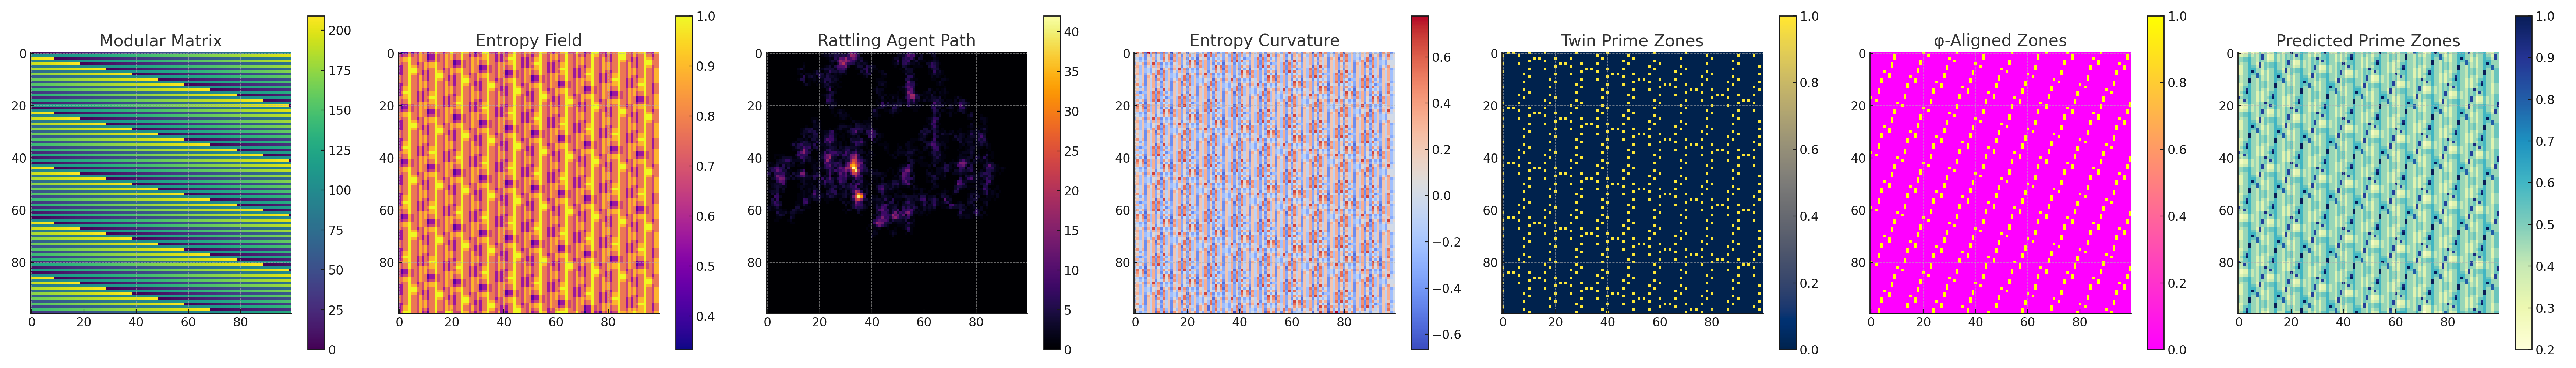
\includegraphics[width=\textwidth]{modular_prime_rattling_analysis.png}
\caption{Visualizations of modular structure, entropy, rattling path density, curvature, twin primes, $\phi$-alignment, and predicted prime zones.}
\end{figure}

\section{Formal Conjecture and Lemmas}
\textbf{Lemma 1 (Prime Entropy Gradient Lemma):}
The entropy field exhibits steep gradients near prime clusters. Rattling agents following these gradients are drawn toward primes.

\textbf{Lemma 2 ($\phi$-Aligned Attractor Lemma):}
The $\phi$-aligned set $A_\phi$ overlaps non-trivially with prime locations due to modular harmonics and continued fraction approximations.

\textbf{Modular Prime Rattling Conjecture:}
Let $P \subset M$ be the set of primes, and $F$ be the predicted field. Then:
\[ \Pr[R(t) \in P] > \Pr[\text{uniform walker} \in P] \iff \nabla F \cdot R(t) > 0 \]

\section{Comparison with Classical Models}
\begin{itemize}
    \item Sieve models are purely divisibility-based; ours is spatial and probabilistic.
    \item Cram\'er and Hardy-Littlewood models assume random primes \cite{hardy2008introduction, granville1995unexpected}; ours leverages emergent field structures.
    \item Riemann Hypothesis relies on complex analysis; our approach is real-valued and modular.
\end{itemize}

\section{Conclusion and Future Work}
We believe our model provides a compelling new lens through which to explore the behavior of prime numbers:
\begin{itemize}
    \item Extend to 3D modular lattices and non-square topologies
    \item Use irrational constants beyond $\phi$ (e.g., $\pi$, $\sqrt{2}$)
    \item Connect entropy curvature with zeroes of the Riemann Zeta function
\end{itemize}

\bibliographystyle{plain}
\bibliography{prime_rattling_refs}

\end{document}
